\subsection{Antennenoszillator}\label{subsec:Antennenoszilator}
Für die Antennenoszillator Schaltung übernahmen wir die bereits im Projekt 5 eingesetzte Colpitts-Oszillator Schaltung. Die aus dem Projekt 5 übernommene Schaltung ist in Abbildung \ref{img:colpitts} gezeigt.

\begin{figure}[h]
	\centering
	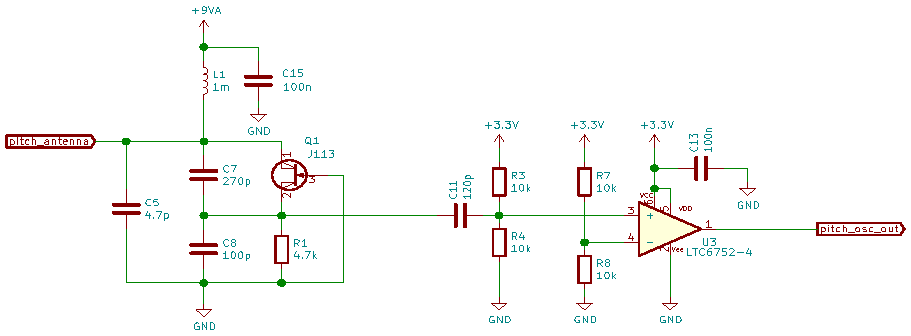
\includegraphics[width=\textwidth]{colpitts.pdf}
	\caption{Schema Antennenoszillator. Links Collpitts-Oszillator,rechts Komparatorschaltung}
	\label{img:colpitts}
\end{figure} 

Es handelt sich dabei um eine Colpitts-Oszillator Schaltung mit einem JFET. Diese Schaltung ist von dem Bauset "Theremin selber bauen" von Franzis übernommen. 
Da der im Bauset verwendete JFET nicht mehr bestellbar ist, verwendeten wir den J113 N-Channel JFET. Die mit LTspice simulierten Werte des J113 glichen stark der original Schaltung, weshalb dieser gewählt wurde. 
Damit das Sinussignal des Antennenoszillator nicht A/D gewandelt werden muss, haben wir entschieden das Sinussignal in ein Rechtecksignal mit gleicher Frequenz zu wandeln. Dies geschieht mithilfe einer Komparatorschaltung. 
Die Komparatorschaltung wird mit \SI{3.3}{V} betrieben da die Logikeingänge des FPGA auf diese Spannung ausgelegt sind. Als Referenzspannung der Komperatorschaltung dient die halbe Versorgungsspannung, welche mit den Widerständen R7 und R8 gebildet wird. 

Als Antenne wird ein Messingrohr verwendet. Dieses ist zwischen der Spule L1 und dem Kondensator C5 verbunden. 

Die Ausgangsspannung des Colpitts-Oszillator ist über den Kondensator C11 entkoppelt. Dies entfernt den DC-Anteil. Der Kondensator C11 und die Widerstände R3 und R4 bilden zusammen einen Hochpass. Damit die Oszillator Frequenz von ca \SI{562}{kHz} das Filter passieren kann ist C11 so gewählt das die Grenzfrequenz des Filters bei ca \SI{265}{kHz} liegt. 

Der Antennenoszillator im Projekt 6 verwendet für die Lautstärke und die Tonhöhenantenne jeweils eine Colpitts-Oszillator Schaltung wie in Abbildung \ref{img:colpitts} gezeigt. Der Antennenoszillator ist mit einem \SI{12} {VDC} Schaltnetzteil gespiessen. Der MC7809 Spannungsregler generiert die \SI{9} {VDC} für die Colpitts-Oszillator Schaltungen. Die \SI{3.3} {VDC} für den Komperator erzeugt der LT1117 Spannungsregler. Bei der Wahl der Spannungsregel ist darauf geachtet worden das die erzeugten Spannungen möglichst Störungsfrei und wenig Rippel aufwiesen. Das gesamte Schema der Schaltung ist im Anhang enthalten.


